% !TEX root = thesis.tex

\chapter{$\zg$+Jets at 100TeV}
\label{chap:100TeV}

	Even though the Large Hadron Collider is still in its infancy there is an ever growing effort to discuss
	where we go next as a high energy collider physics community.  A wide range of options have been put forward
	including the linear colliders Compact Linear Collider (CLIC) \cite{Abramowicz:2013tzc} and the International
	Linear Collider (ILC) \cite{BrauJames:2007aa}.  While both of these machines are designed to be precision
	electron-positron linear colliders they have very different designs; CLIC would operate at around a
	centre-of-mass energy of $3$~TeV and use cutting edge accelerating technology whereas the ILC would collide
	at $0.5$~TeV (with a possible upgrade to $1$~TeV).

	However, there are other suggestions on the table.  Of particular interest for this work is the prospect
	of a hadronic Future Circular Collider (FCC-hh).  There are other possible initial states such as
	hadron-lepton or a lepton-lepton being discussed but for obvious reasons it is the FCC-hh which we will
	focus on here.

	One particularly exciting scenario is that of a \htev hadronic collider housed in an extended tunnel
	approximately $100$~km in circumference at the CERN site in Geneva.  Such a machine would make an
	excellent `discovery machine' since it would cover a vast range in partonic centre-of-mass energies.
	The energies probed here would be orders of magnitude higher than ever seen at a hadronic collider
	and so this would be an invaluable test of high scale QCD.  Similarly to physics at the current LHC
	the dominant background would be QCD in nature and so in order for us to be able to extract useful
	information about potential new physics we would need to be able to model this QCD background with
	incredible precision.  Current state-of-the-art for many QCD processes is still limited to next-to-leading
	order in $\alpha_s$ although progress is being made towards improving this to next-to-next-to-leading
	order in some key physics processes, for example Higgs production via gluon fusion is known at N3LO \cite{Anastasiou:2015ema}.
	However, as in the preceding chapters we will instead investigate the effects of the higher-order
	logarithmically enhanced contributions to the perturbative series.  As discussed in chapter \ref{chap:theory}
	these terms are not all captured by NNLO (or any fixed-order scheme $\text{N}^m$LO for that matter).

	The results of chapters \ref{chap:Zs} and \ref{chap:ATLAS} clearly show that these effects are already important
	at a the \stev for both dijets and $\zg$+dijets respectively.  We therefore expect that at a \htev FCC-hh we would
	see a greater effect from the terms enhanced in the High Energy limit beyond a fixed-order only prediction.

	Here we present a study of $\zg$+dijets at a centre-of-mass energy of \htev.  The final state cuts
	are outlined in table~\eqref{tab:atlascuts100}.  For each figure we show the equivalent result calculated
	at \stev with a jet $p_T$ cut of $30$~GeV (which was found to be in excellent agreement with data) as
	well as the \htev predictions for jet cuts of $30$~GeV, $60$~GeV and $100$~GeV.  The jet cut choice
	is an interesting problem since it the best variable for weeding out physics other than the hard
	perturbative scatter.  For example, even at the \stev LHC a QCD study with a jet cut of, say,
	$10$~GeV would be as much a test of our theoretical understanding of perturbative physics as it would
	a test of our descriptions for parton showers, multiple parton interactions and underlying event.
	While this is a perfectly valid analysis to do it is \emph{not} the best choice if our aim is to
	improve our understanding of perturbative QCD.  The same argument applies for a \htev collider
	only more so!  As we go to increasingly higher centre-of-mass energies we may need to raise our
	jet cuts so as to ensure the data we hope to describe is as unpolluted as possible.  Each figure
	also shows the ratio of the \htev prediction to the \stev prediction to emphasise any features
	which may otherwise be hard to see - such as changes in shape.

	\begin{table}[bth]
	  \centering
	  \begin{tabular}{|l|c|}
	    \hline
	    Lepton Cuts & $p_{T\ell}>20$~GeV, \; $|\eta_\ell|<2.5$ \\
	    & $\Delta R^{\ell^+\ell^-} > 0.2$, \; $66$~GeV $\leq m^{\ell^+\ell^-} \leq
	      116$~GeV \\ \hline
	    % $7$~TeV Jet Cuts (anti-$k_T$, 0.4) & $p_{Tj}>$ {\color{red}$30$~GeV} \\
	    % &  $|y_j|<4.4$, \;$\Delta R^{j\ell} >0.5$,  \\
	    $100$~TeV Jet Cuts (anti-$k_T$, 0.4) & $p_{Tj}>$ {\color{red}$30$~GeV}, {\color{green}$60$~GeV}, {\color{blue}$100$~GeV} \\
	    &  $|y_j|<4.4$, \;$\Delta R^{j\ell} >0.5$,  \\
	\hline
	  \end{tabular}
	  \caption{Cuts applied to theory simulations for the \htev
	    $Z$-plus-jets analysis results shown in Figs.~\eqref{fig:100tev_12a}--\eqref{fig:100tev_10b}.}
	  \label{tab:atlascuts100}
	\end{table}

	We begin by discussing what is by far the most uninteresting figure in this thesis (at least at first glance!).
	Fig.~\ref{fig:100tev_12a} shows the differential distribution with respect to the azimuthal separation of the
	two leading jets in $p_T$, $\Delta\phi_{j1, j2}$.  It is clear that although the cross-section of the \htev
	result is significantly greater than that of the \stev result the increase in cross-section is uniform
	throughout the range of $\Delta\phi_{j1, j2}$ - this is clear from the ratio.  What makes the
	uninteresting fig.~\ref{fig:100tev_12a} interesting is that if QCD behaved exactly the same at \htev
	as it did at \stev we would expect all of the plots in this chapter to have a ratio line which
	was a perfectly straight line which merely reflected the increase in cross-section.  However, this
	turns out not to be the case.

	\begin{figure}[bth]
		\centering
		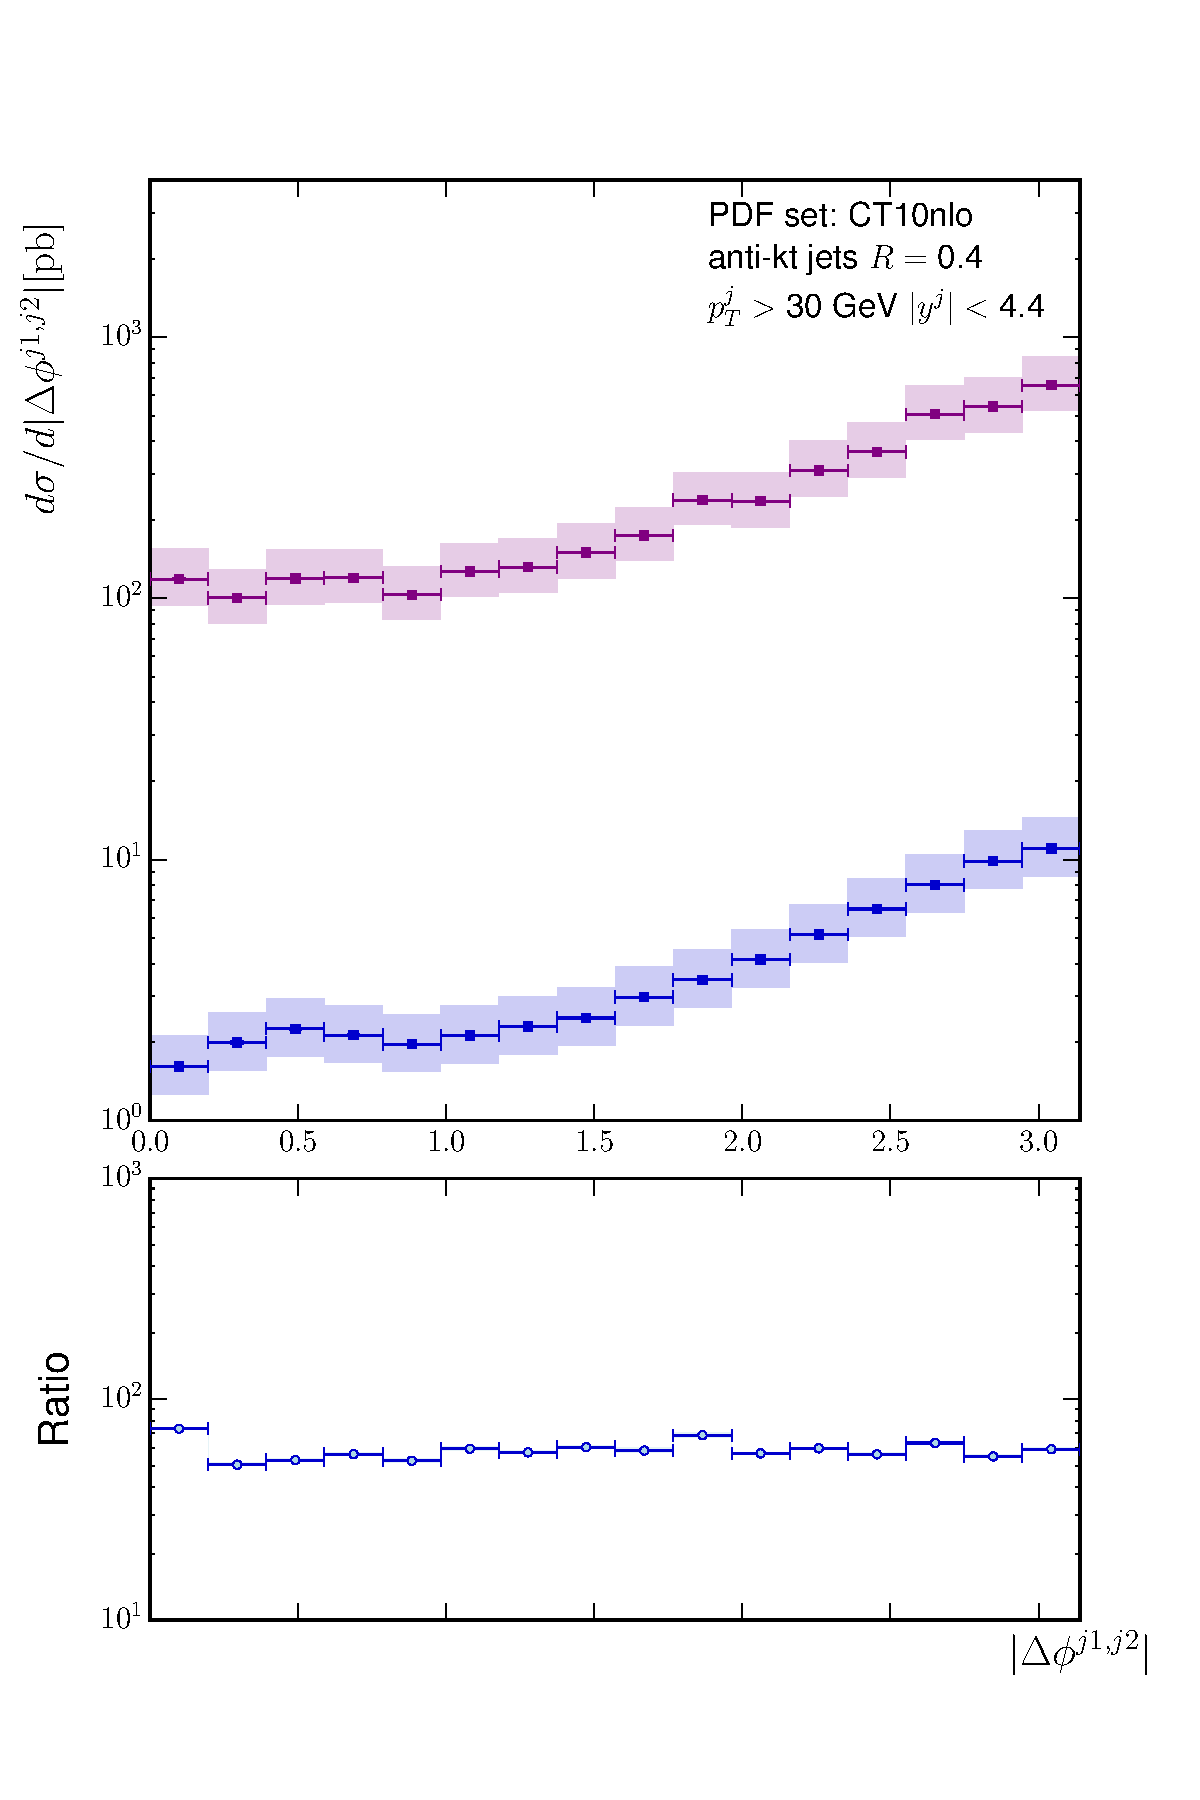
\includegraphics[width=0.7\linewidth]{ATLAS_Z_100TeV_12a}
		\caption{The differential cross-section for $\zg$ plus inclusive dijets as a
		function of the azimuthal separation of the dijet system shown for centre-of-mass
		energies of 7TeV (blue) and 100TeV (pink).}
		\label{fig:100tev_12a}
	\end{figure}

	Fig~\ref{fig:100tev_2a} shows the inclusive $\zg$+dijets cross-section as a function of the number
	of jets, $N_{\text{jet}}$.  Once again we see that the total integrated cross-section grows as we
	go to higher energy but we also see that the relative contribution to the cross-section increases
	as we go to higher jet multiplicity.  This is direct evidence that the convergence of the
	QCD perturbative expansion worsens as we go to higher energy.  Clearly then resummation effects
	such as those described by \hej become more important at a prospective FCC-hh machine and will need
	to be included not only in order to understand the QCD background well enough to extract and
	study new physics but also in order for precision tests of QCD.

	\begin{figure}[bth]
		\centering
		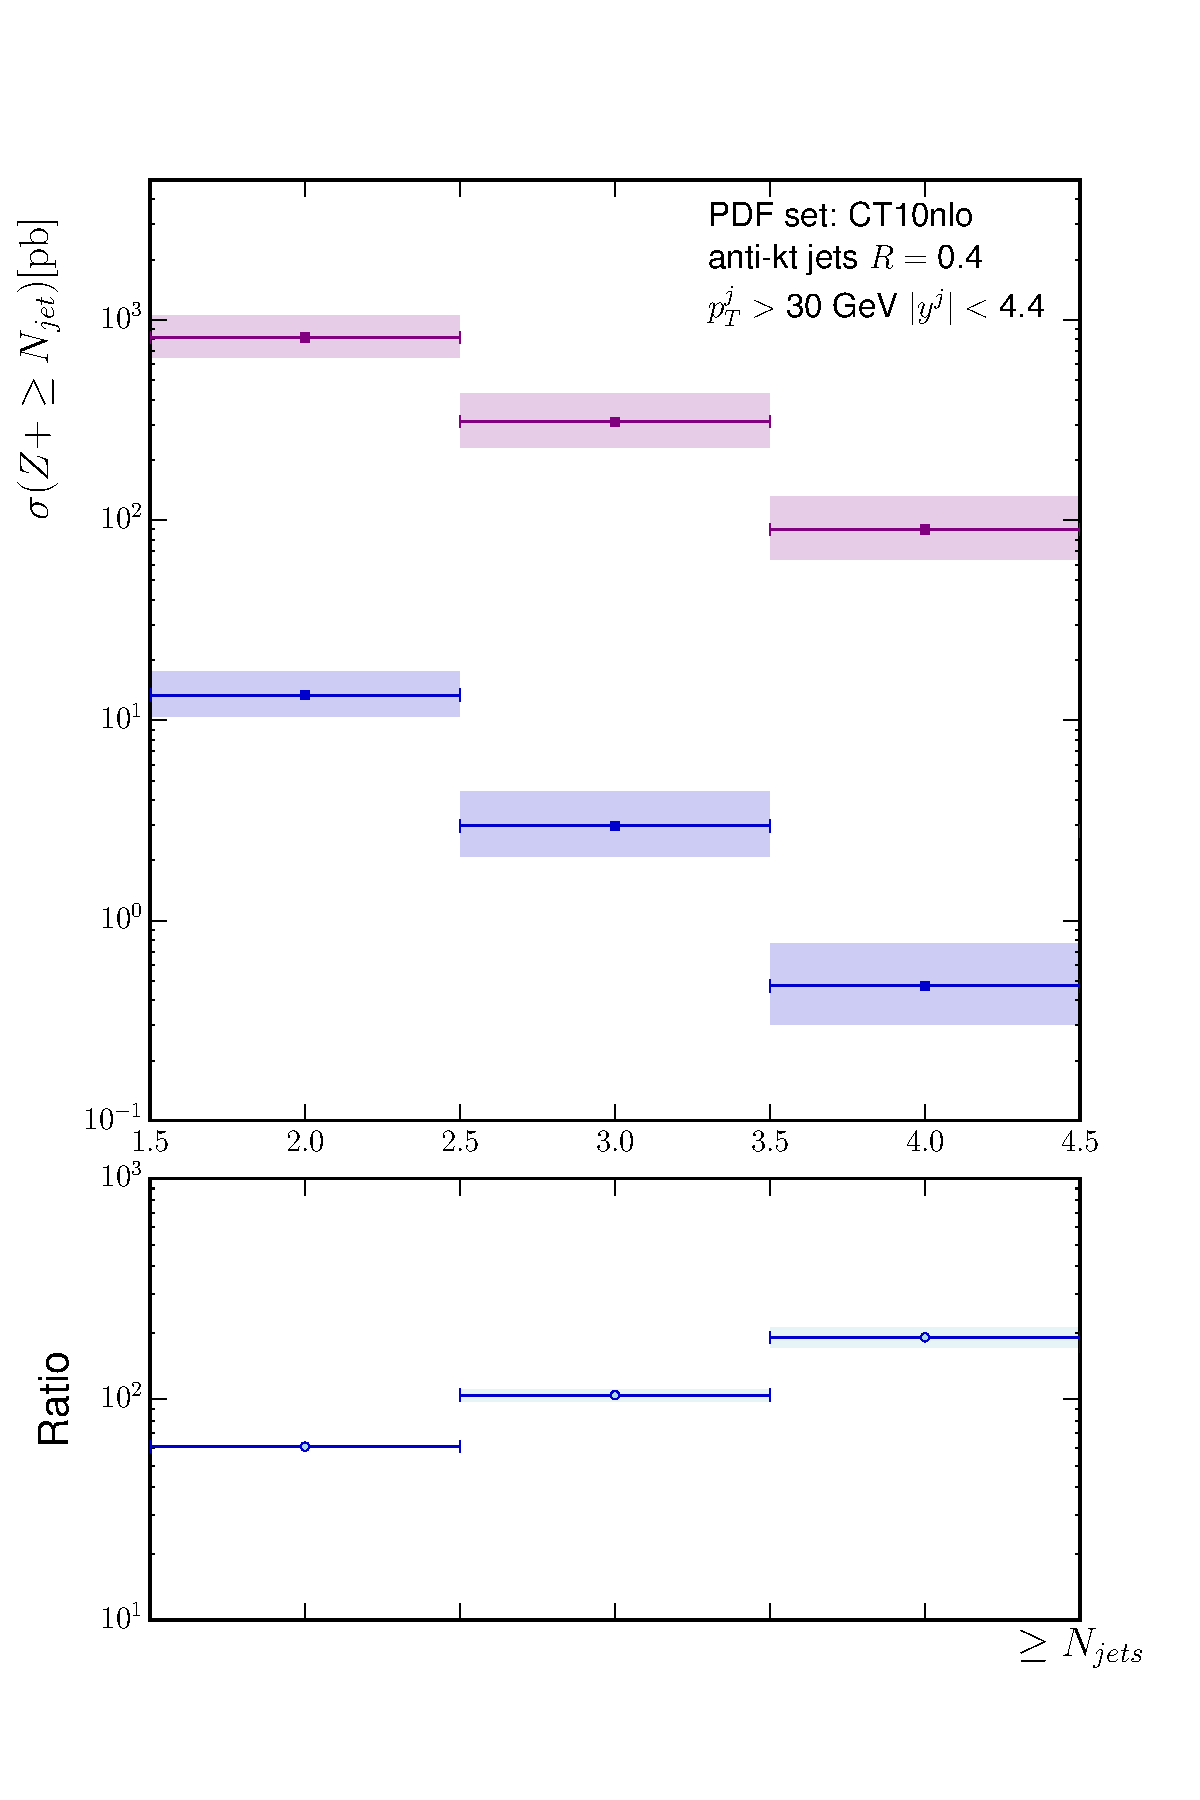
\includegraphics[width=0.7\linewidth]{ATLAS_Z_100TeV_2a}
		\caption{The cross-section for $\zg$ plus inclusive dijets as a function of the number of
		jets, $N_{\text{jet}}$, shown for centre-of-mass energies of 7TeV (blue) and 100TeV (pink).}
		\label{fig:100tev_2a}
	\end{figure}

	Fig~\ref{fig:100tev_11a} shows the differential distribution with respect to the absolute value of the
	rapidity span between the two leading jets in $p_T$, $\Delta y^{j1, j2}$.  We see that as we go to
	large rapidity gaps between the dijets the relative increase in the cross-section grows by almost a
	factor or $10$.  This is precisely

	\begin{figure}[bth]
		\centering
		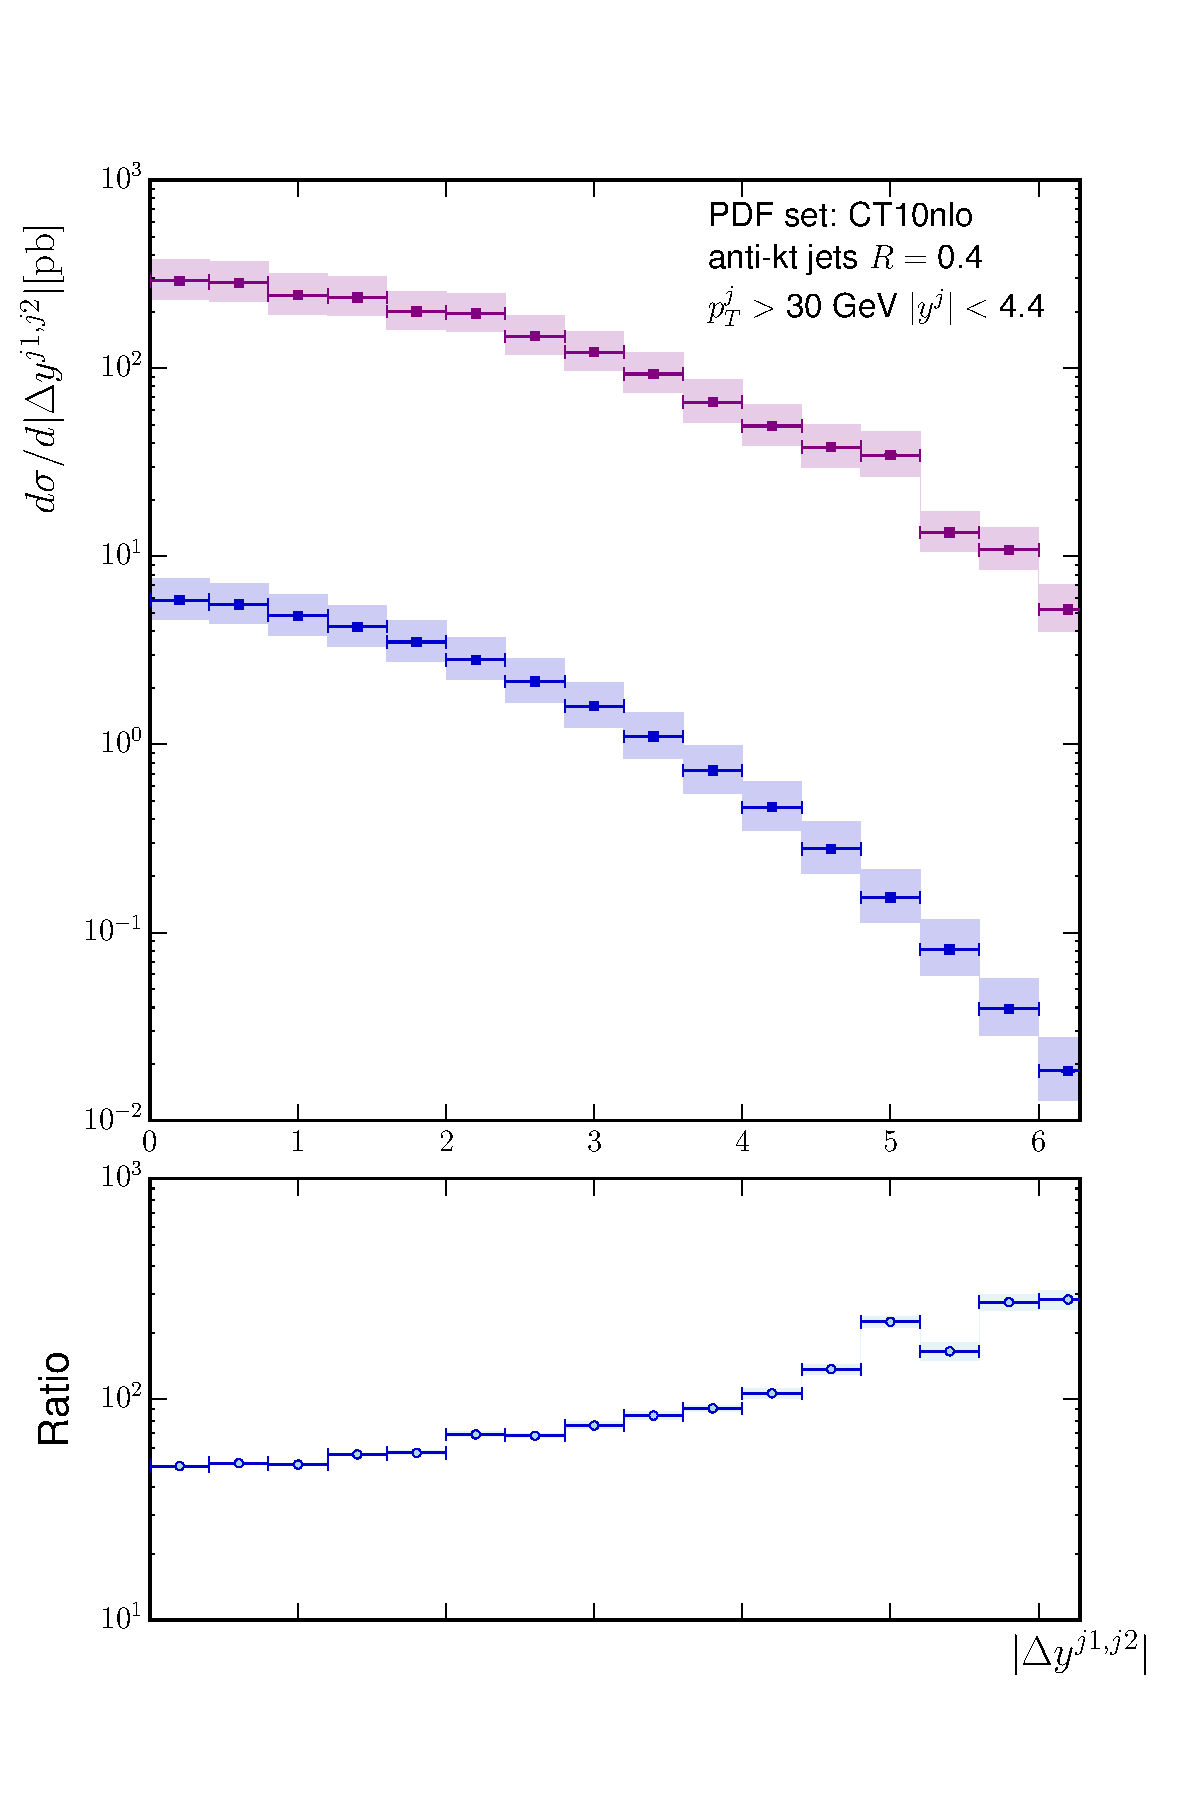
\includegraphics[width=0.7\linewidth]{ATLAS_Z_100TeV_11a}
		\caption{The differential cross-section for $\zg$ plus inclusive dijets as a function of the absolute value of the
		         rapidity gap between the dijets, $\Delta y^{j1, j2}$ shown for centre-of-mass energies of 7TeV (blue) and
		         100TeV (pink).}
		\label{fig:100tev_11a}
	\end{figure}

	Fig. (\eqref{fig:100tev_11a}) notes:

	\begin{itemize}
		\item dy plot,
		\item O(10) increase in cross-section as we go to large rapidities,
		\item More energy in initial state means we can get more jets further into the outer regions of y-space,
		\item The increase seen is \emph{exactly} the large logs we capture at play
	\end{itemize}

	\begin{figure}[bth]
		\centering
		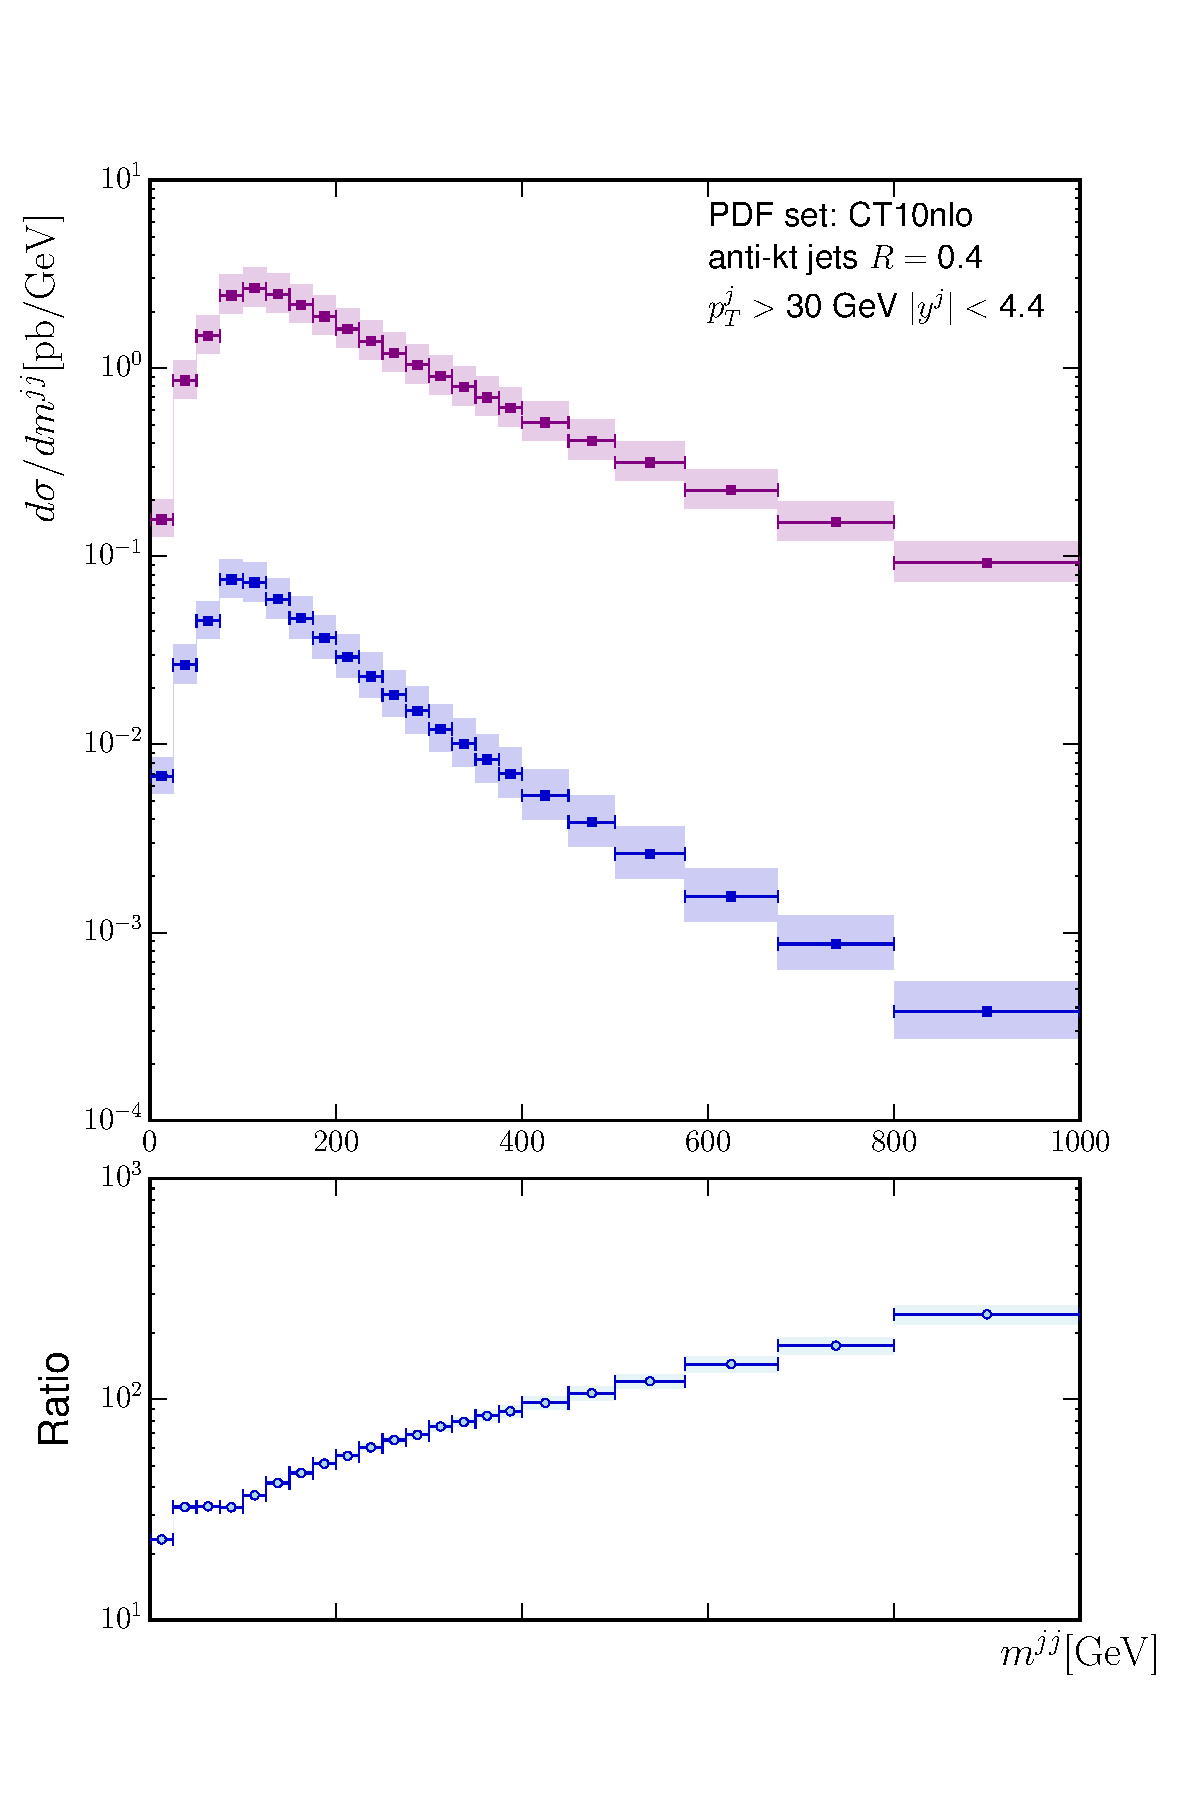
\includegraphics[width=0.7\linewidth]{ATLAS_Z_100TeV_11b}
		\caption{The differential cross-section for $\zg$ plus inclusive dijets as a function of the invariant mass
		         of the dijets, $m^{jj}$, shown for centre-of-mass energies of 7TeV (blue) and 100TeV (pink).}
		\label{fig:100tev_11b}
	\end{figure}

	Fig. (\eqref{fig:100tev_11b}) notes:

	\begin{itemize}
		\item $dm_jj$ plot,
		\item O(10) increase in cross-section as we go to large invariant masses,
		\item Invariant masses again correlate with the logs we resum (show this explicitly if you havent already),
		\item Similar to fig. (\eqref{fig:100tev_11a})
	\end{itemize}

	\begin{figure}[bth]
		\centering
		\begin{subfigure}[b]{0.48\textwidth}
			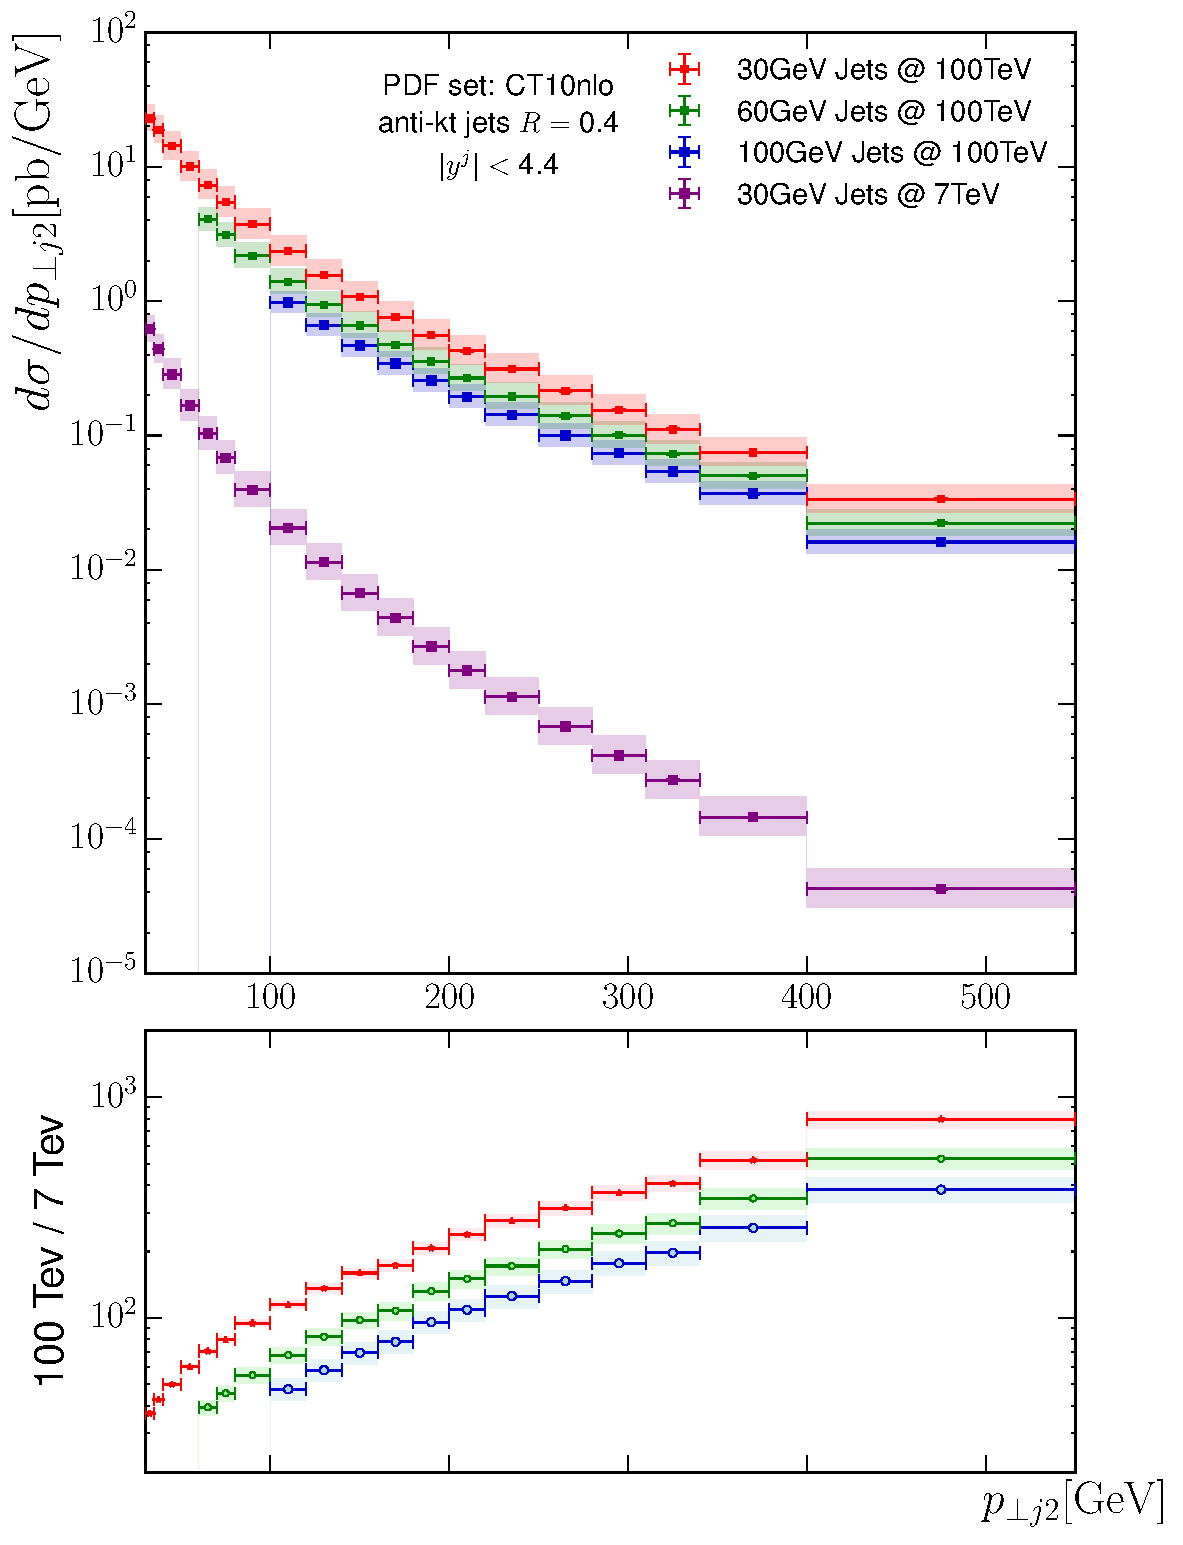
\includegraphics[width=\textwidth, height=1.3\textwidth]{ATLAS_Z_100TeV_5b}
			\caption{}
			\label{fig:100tev_5b}
		\end{subfigure}

		\begin{subfigure}[b]{0.48\textwidth}
			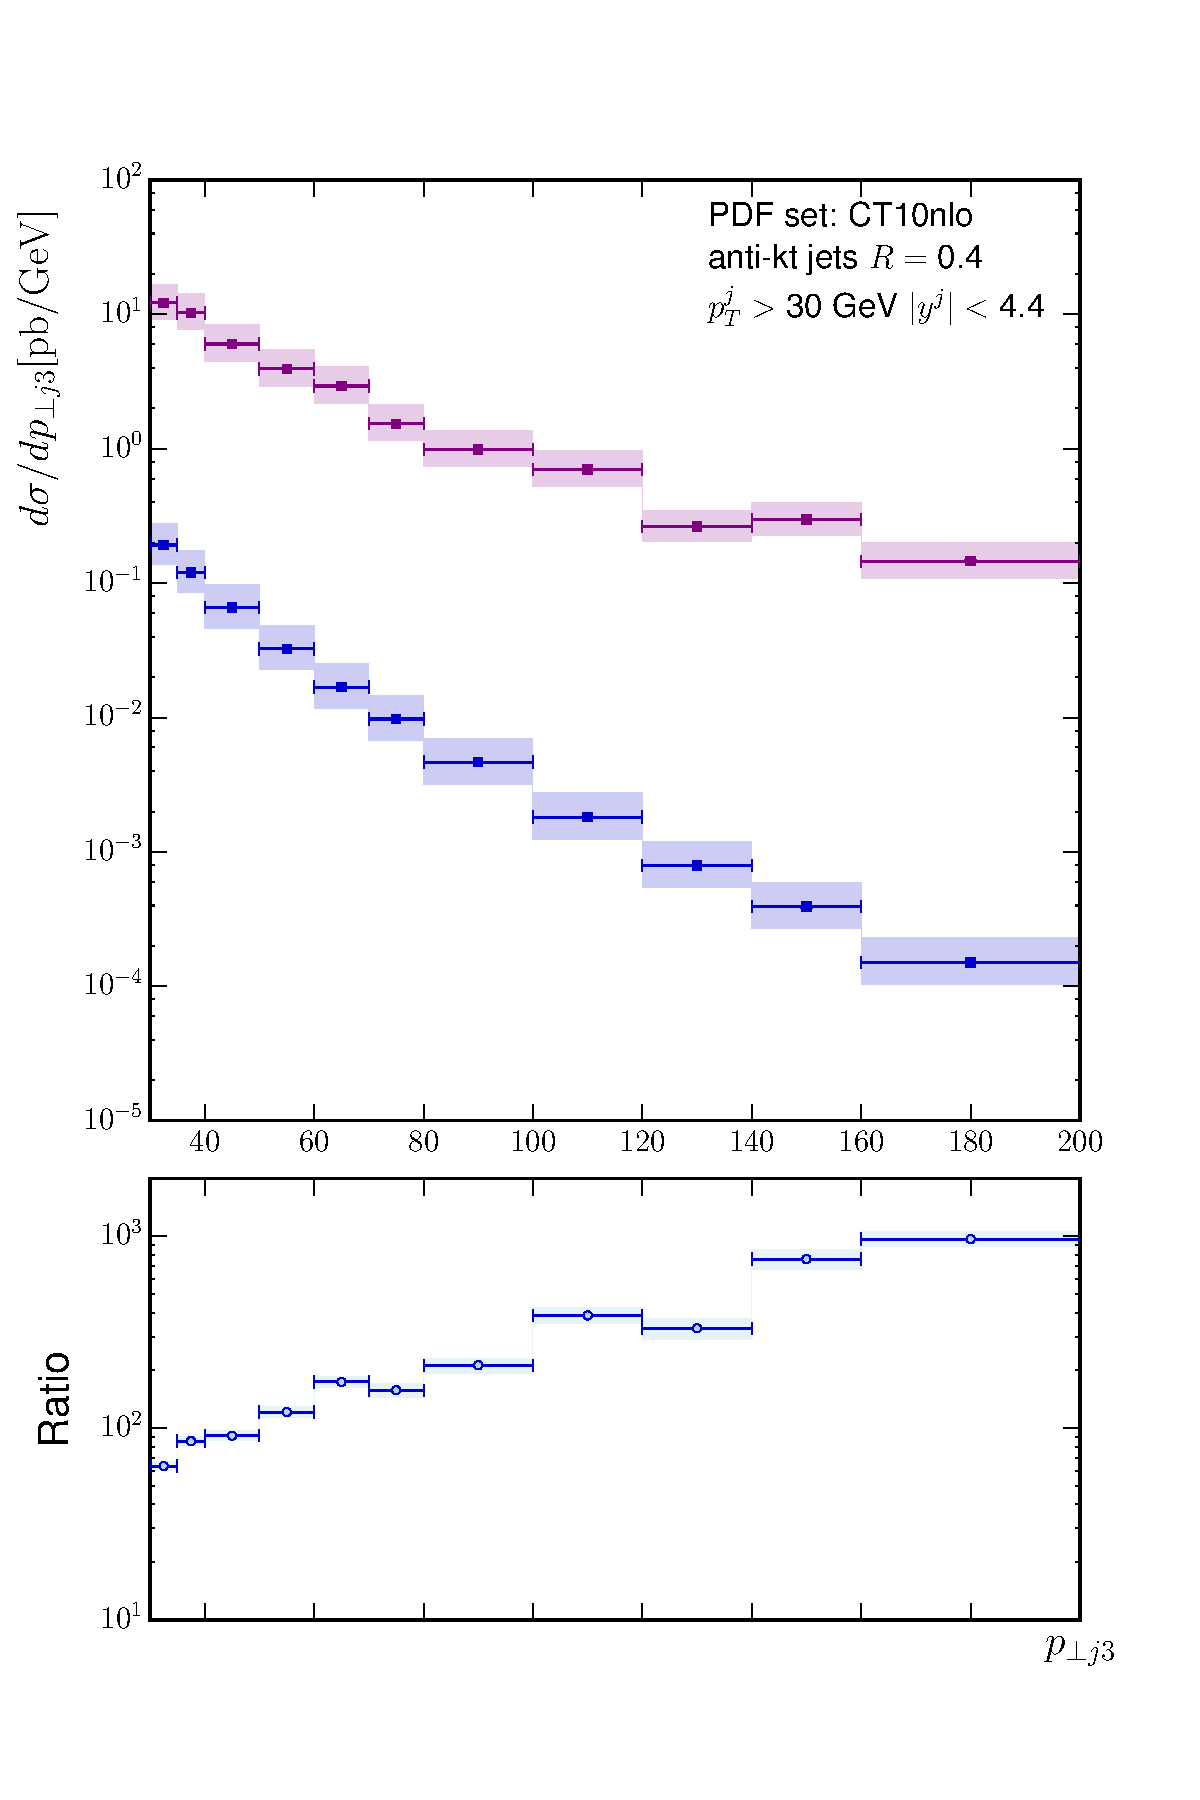
\includegraphics[width=\textwidth, height=1.3\textwidth]{ATLAS_Z_100TeV_6a}
			\caption{}
			\label{fig:100tev_6a}
		\end{subfigure}
		~
		\begin{subfigure}[b]{0.48\textwidth}
			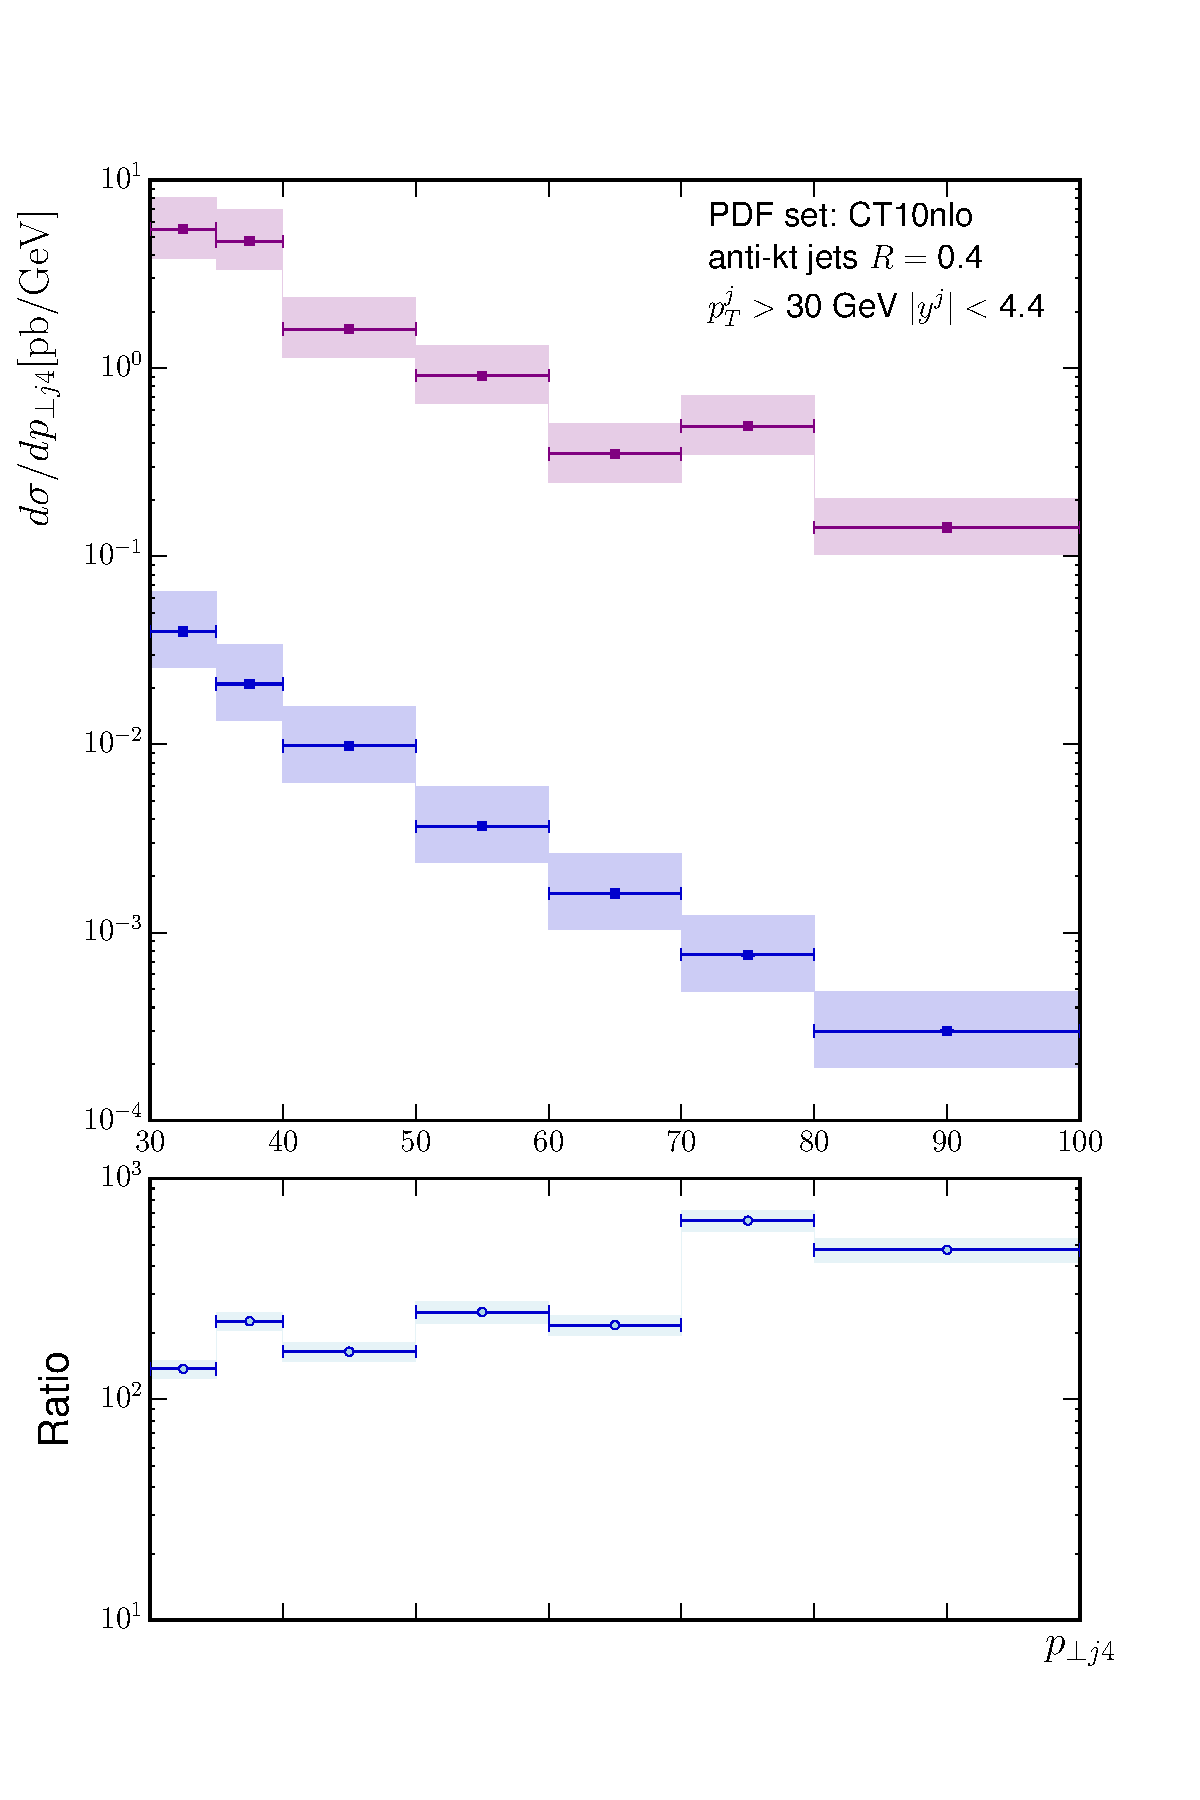
\includegraphics[width=\textwidth, height=1.3\textwidth]{ATLAS_Z_100TeV_6b}
			\caption{}
			\label{fig:100tev_6b}
		\end{subfigure}
		\caption{The differential cross-section for $\zg$ plus inclusive dijets as a function of the transverse momentum
		         of the first, second and third leading jets in $p_T$ shown in fig. \eqref{fig:100tev_5b}, \eqref{fig:100tev_6a}
		         and \eqref{fig:100tev_6b} respectively and for centre-of-mass energies of 7TeV (blue) and 100TeV (pink).}
	\end{figure}

	Fig. (\eqref{fig:100tev_5b}-\eqref{fig:100tev_6b}) notes:

	\begin{itemize}
		\item pT distributions,
		\item Heavy tails...soooo?
		\item More energy in initial state means we can get more jets further into the outer regions of y-space,
		\item What effect would a shower have on these distributions?  Plenty of spare pT to radiate.
	\end{itemize}

	\begin{figure}[bth]
		\centering
		\begin{subfigure}[b]{0.48\textwidth}
			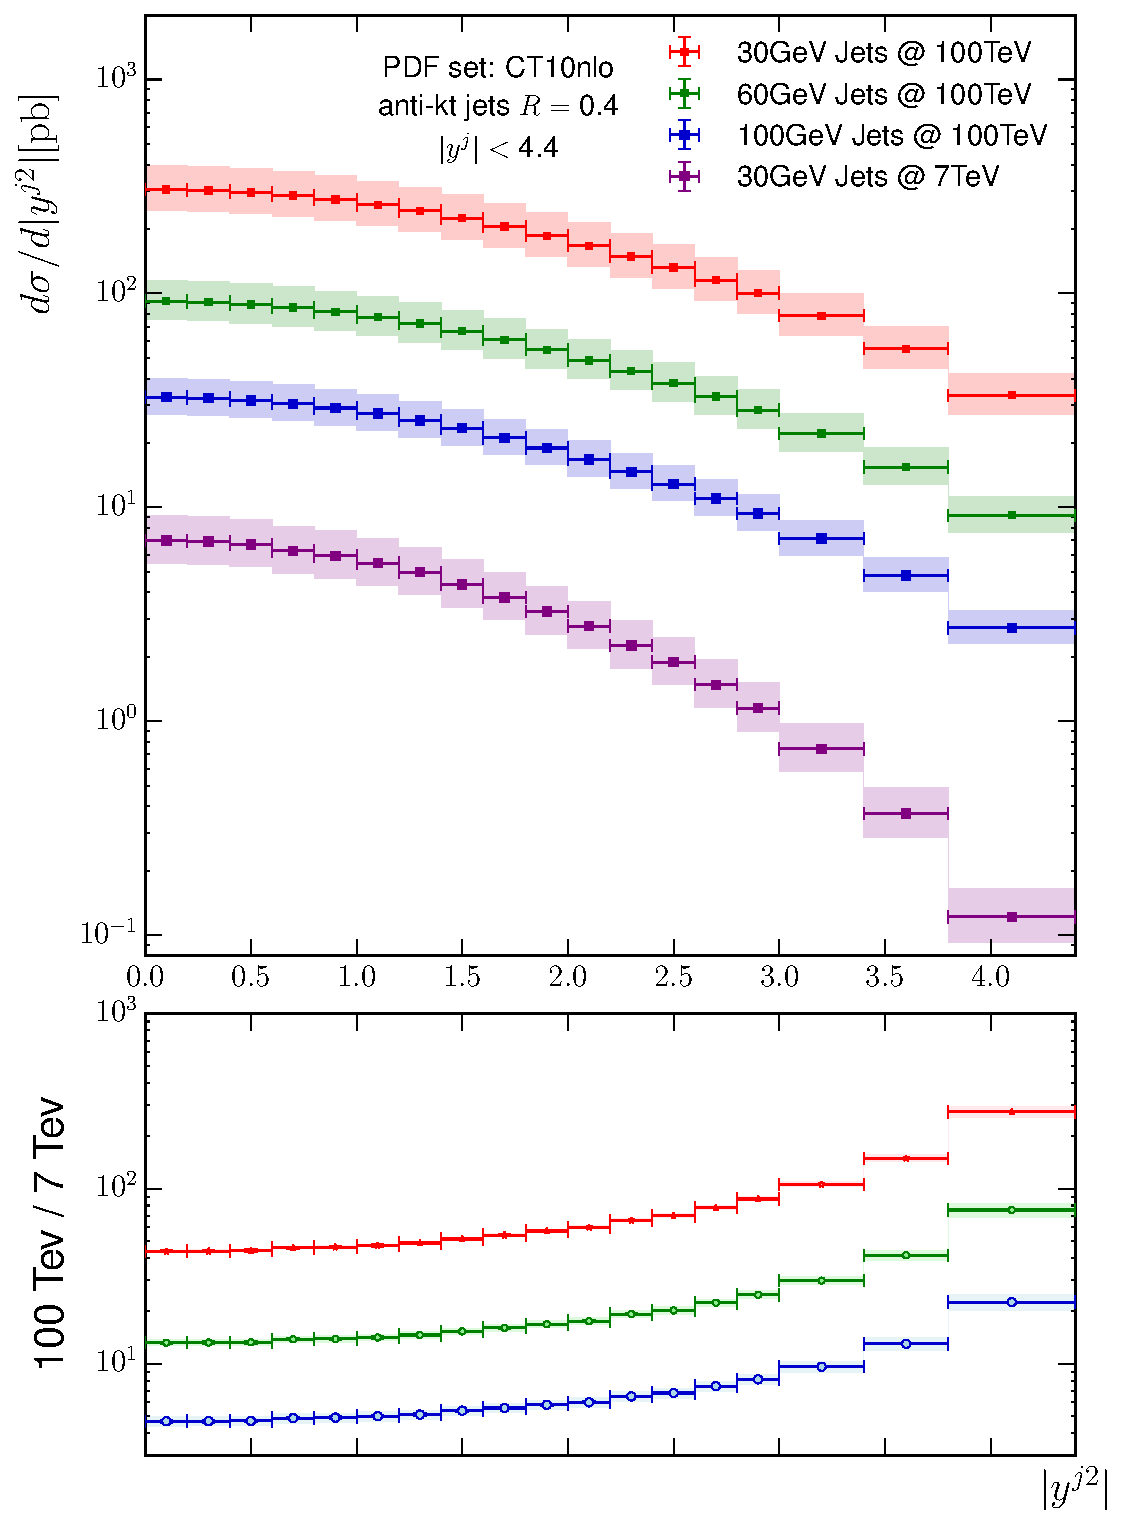
\includegraphics[width=\textwidth, height=1.3\textwidth]{ATLAS_Z_100TeV_9b}
			\caption{}
			\label{fig:100tev_9b}
		\end{subfigure}

		\begin{subfigure}[b]{0.48\textwidth}
			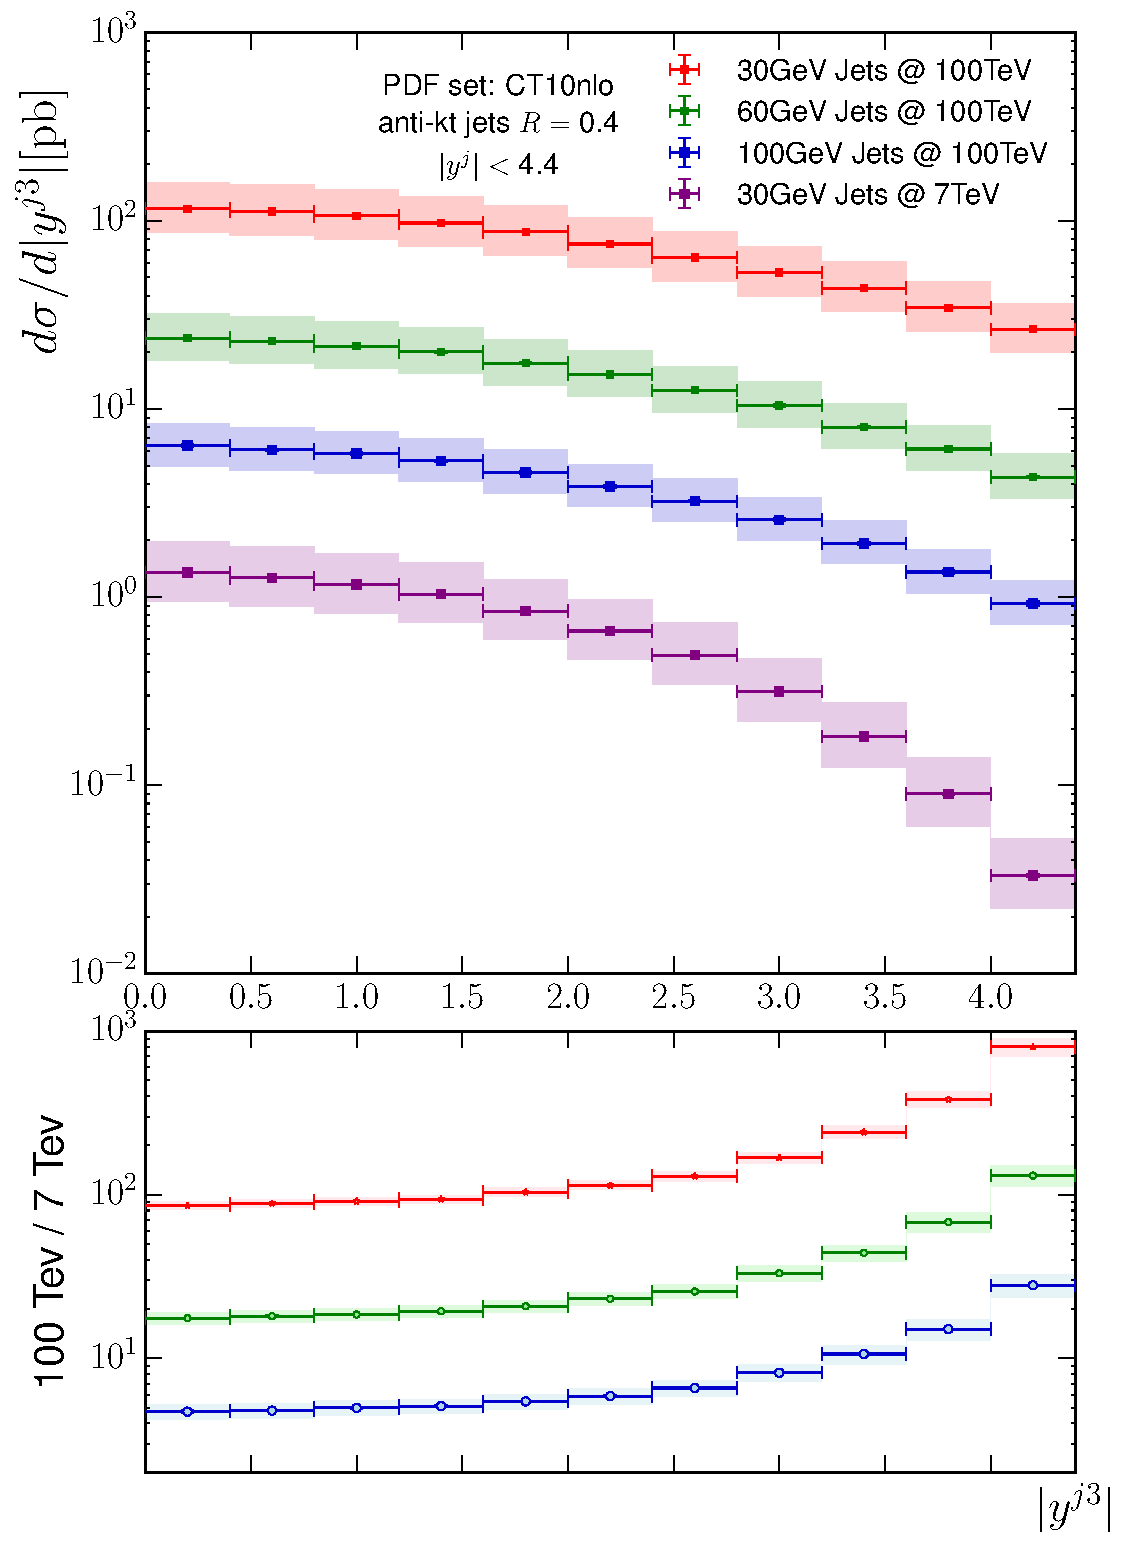
\includegraphics[width=\textwidth, height=1.3\textwidth]{ATLAS_Z_100TeV_10a}
			\caption{}
			\label{fig:100tev_10a}
		\end{subfigure}
		~
		\begin{subfigure}[b]{0.48\textwidth}
			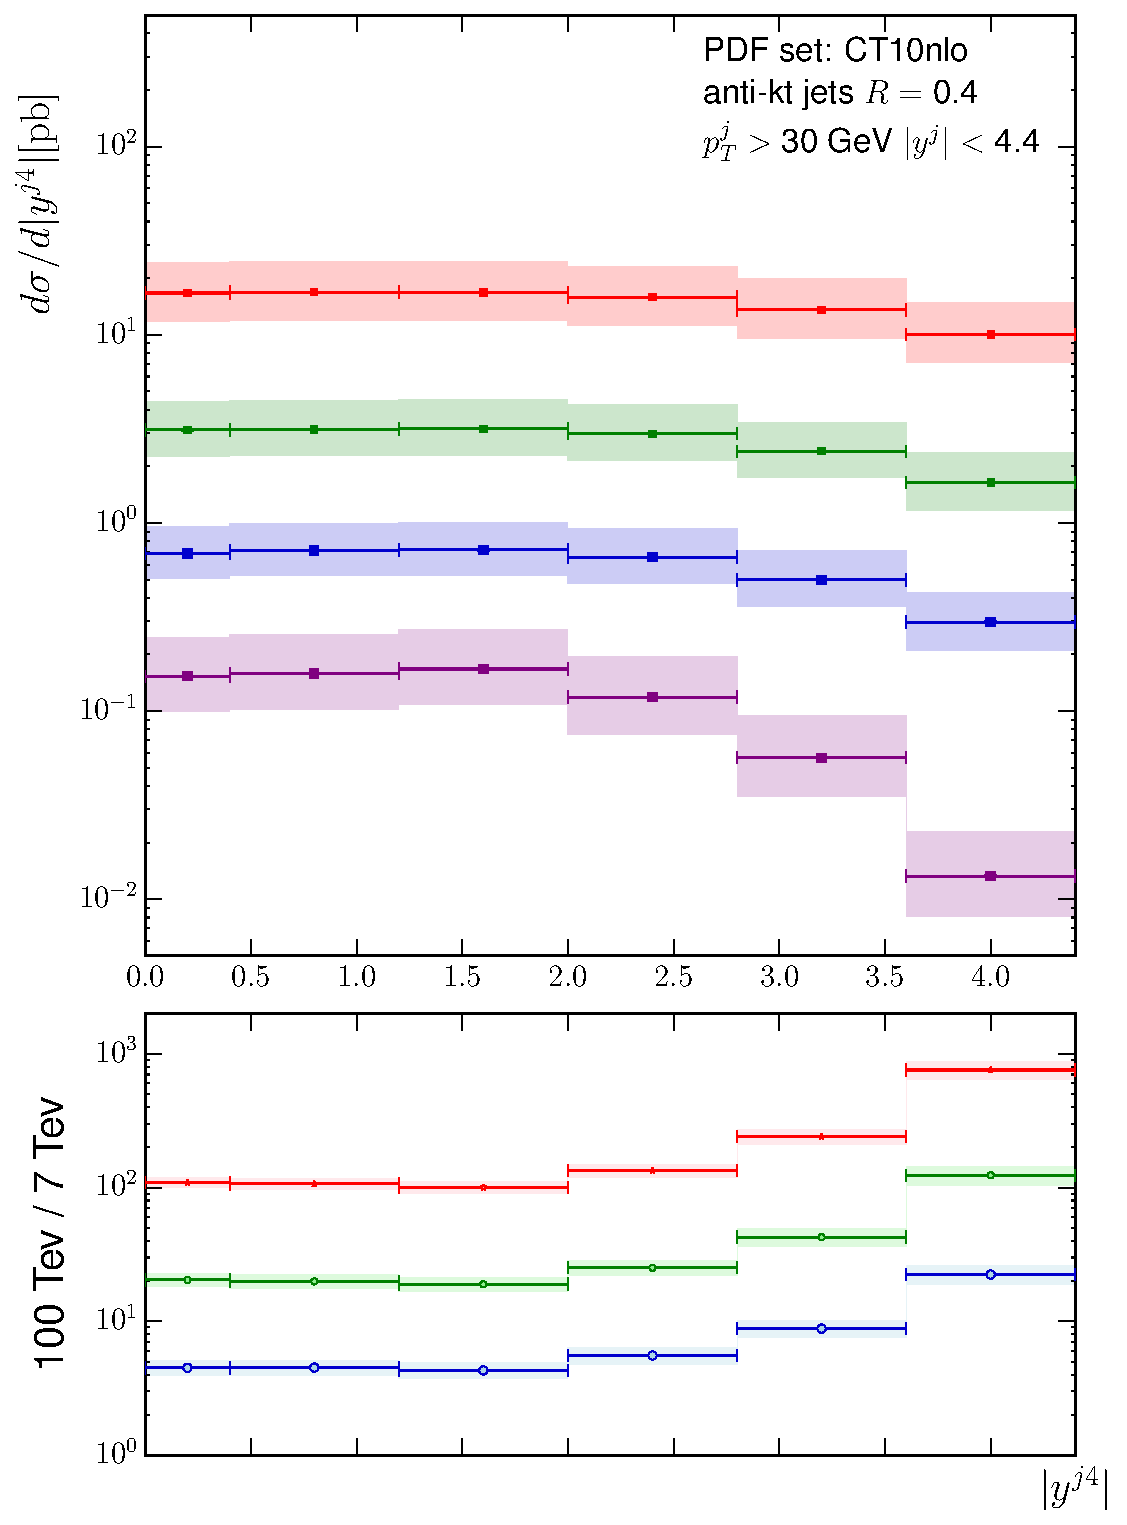
\includegraphics[width=\textwidth, height=1.3\textwidth]{ATLAS_Z_100TeV_10b}
			\caption{}
			\label{fig:100tev_10b}
		\end{subfigure}
		\caption{The differential cross-section for $\zg$ plus inclusive dijets as a function of the absolute value of the rapidity
		         of the first, second and third leading jets in rapidity shown in fig. \eqref{fig:100tev_9b}, \eqref{fig:100tev_10a}
		         and \eqref{fig:100tev_10b} respectively and for centre-of-mass energies of 7TeV (blue) and 100TeV (pink).}
	\end{figure}

	Fig. (\eqref{fig:100tev_9b}-\eqref{fig:100tev_10b}) notes:

	\begin{itemize}
		\item Not much more to say about these - mostly covered in dy plots,
	\end{itemize}

